
\section*{Part B, Problem 2 K-NN (15 pts) (Weixiang)}
\begin{enumerate}
	\item \textbf{(9 points)}
	For each of the following figures, we are given a few data points in
	2-d space,each of which is labeled as either positive (blue) or
	negative (red). Assuming that we are using L2 distance as a distance
	metric, draw the decision boundary for 1-NN for each case. In other words, with your decision boundary, the new test data can be classified into corresponding categories. As an example, we draw the decision boundary for you with figure (a).
	
	\begin{figure*}[h!]
		\centering
		\begin{tabular}{cccc}
			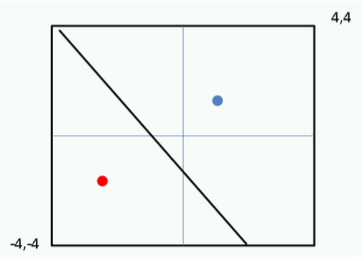
\includegraphics[width=.25\columnwidth]{pa.png}& 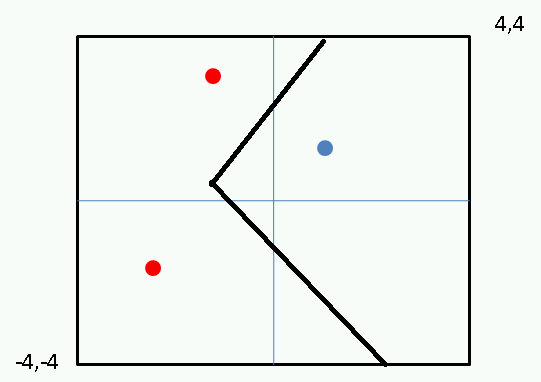
\includegraphics[width=.25\columnwidth]{pb.png}& 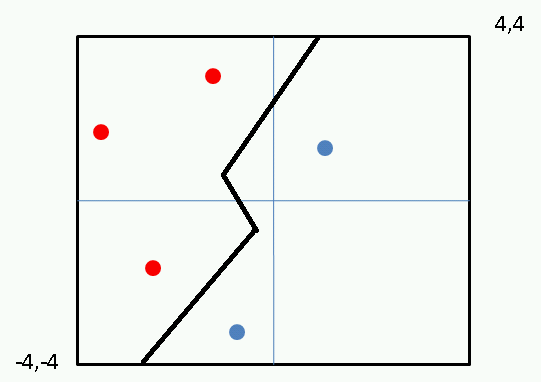
\includegraphics[width=.25\columnwidth]{pc.png}&
			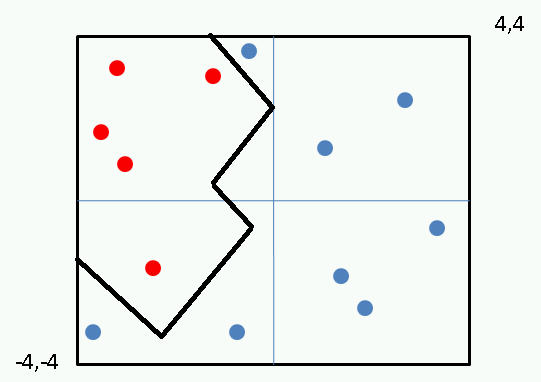
\includegraphics[width=.25\columnwidth]{pd.png}\\
			(a) & (b) & (c) & (d)
		\end{tabular}
	\end{figure*}
	
	
	\item \textbf{(3 points)} In class we have mentioned that K-NN is a \emph{lazy}
	classifier. Do we \emph{always} need to store all training data to build our 1-NN classifier when we have $n (n\geq3)$ points? Why? Is there a case that you must store all training data points (i.e., use all training data points when doing the classification)? Why?
	\\\textbf{Answer:}\\
	No, we don't need to store all data points for 1-NN classifier, because some points are far from the decision boundary, and the classification of the region around these points can be determined by the points near decision boundary. If all points are near the decision boundary, we must store all training data points.
	
	\item \textbf{(3 point)}
	Decision tree classfier requires the availability of all training data to build the tree. Thus when a new training data point comes in, it might influence the structure of the decision tree. Does K-NN also suffer from this problem and why (explian in 1-2 sentences)? 
	\\\textbf{Answer:}\\
	With the increment of K, the decision boundary relies on more and more training data and even the whole dataset. If this happens, K-NN also suffers from this problem.
	
\end{enumerate}
\newpage
